\documentclass[12pt,a4paper,openany]{book}
%------------------------------------------------------------------------------------------------------------------------------------------------------------------------------------------------------------------------------
% PACKAGES
%--------------------------------------------------------------------------------------------------------------------------------------------------------------------------------------------------------------------------------

% Selección de idioma
\usepackage[spanish]{babel}

% algo
\usepackage[utf8]{inputenc}

% Tablas
\usepackage{tabularx}
\usepackage{multirow}
\usepackage{multicol} 
\usepackage{booktabs}%\usepackage{booktabs, calc} %This is the package to use to have nice-looking tables. More documentation on the tables in LateX: https://www.tug.org/pracjourn/2007-1/mori/mori.pdf
\usepackage{threeparttable} 

\usepackage{lmodern}
\usepackage{booktabs}
\usepackage{pgfplots}

\graphicspath{{../figuras/}}

\begin{document}
	
	%---------------------------------------------------------------------------
	% TITLE PAGE
	%---------------------------------------------------------------------------
	\doublespacing
	
	\title{Boletín COVID-19}
	\author{Autores}
	
	\date{}

	%\maketitle
	
	
	%\thispagestyle{empty}\baselineskip1.385\baselineskip \newpage{}
	
	\pagestyle{plain}\pagenumbering{arabic}
	
	%insertar el cover
	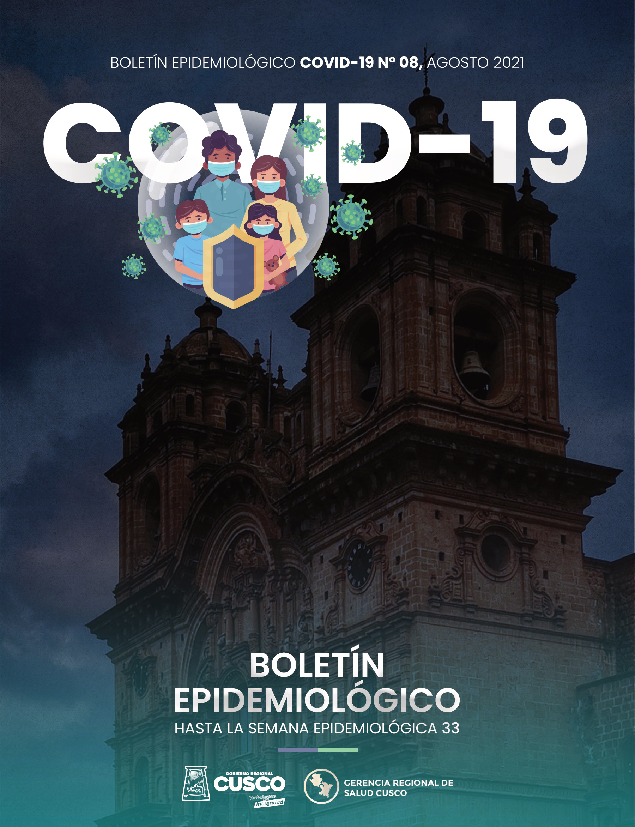
\includepdf[pages={1}]{../editorial/cover_boletin_8.pdf}
	\clearpage
	
	\pagestyle{plain}\pagenumbering{arabic}
	
	\clearpage
	
	
	\begin{center}
		{\large Gerencia Regional de Salud}
		
		\textbf{MSP. Javier Ramírez Escóbar}
		
		Gerente Regional \vspace{1.0cm}
		
		Dirección Ejecutiva de Inteligencia Sanitaria
		
		\textbf{MSP. Darío Francisco Navarro Mendoza}
		
		Director
		
		\vspace{1.5cm}
\noindent
\begin{minipage}[t]{.45\textwidth}
	\centering
	Dirección de Epidemiología e Investigación  \\
	\textbf{MSC. Fátima R. Concha Velasco}\\
	Directora \vspace{1.0cm}\\
	% Por orden alfabético del apellido
	\textit{Equipo de Epidemiología e Investigación }\vspace{.5cm}\\
	Econ. Karen Yorka Aguilar Zuñiga \\
	M.C Edwards Adrian Aguirre Valenzuela \\
	Lic. Nadia Isabel Cáceres Pillco \\
	Econ. Johar Jurimao Cassa Avendaño \\
	TAP. Edgar Waldo Capcha Salcedo \\
	M.S.P. Pablo Fidel Grajeda Ancca \\
	M.C. Katia Luque Quispe \\
	M.C. Ana Gabriela Eulalia Moncada Arias \\
	Lic. Enf. Ruth Nelly Oscco Abarca \\
	Lic. Enf. Guinetta Margarita Yabar Herrera \vspace{1.5cm}\\	
\end{minipage}
\hfill
\noindent
\begin{minipage}[t]{.45\textwidth}
	\centering
	Dirección de Estadística, Informática y Telecomunicaciones\\
	\textbf{Ing. Abel Rimasca Chacón} \\
	Director \vspace{1.0cm} \\
	% Por orden alfabético del apellido
	\textit{Equipo de Estadística, Informática y Telecomunicaciones} \vspace{.5cm} \\
	Ing. Iván Atayupanqui Rondón \\
	Ing. Miguel Ángel Campana Alarcón \\
	Ing. Uriel Lacuta Farfán \\
	Ing. Jorge Fernando Lovatón Ramos \\
	Ing. Danny Robert Moscoso Sánchez \\
	Lic. Ray Milton Valderrama Álverez \vspace{1.5cm}\\
\end{minipage}
Secretaria: Sra. Ruth Baca Mendoza
	\end{center}
\let\cleardoublepage\clearpage
	\tableofcontents
	\listoffigures
	\listoftables
	
	%\mainmatter
	%---------------------------------------------------------------------------
	% CAPÍTULO: EDITORIAL
	%---------------------------------------------------------------------------
	
	\chapter*{Editorial}
	\addcontentsline{toc}{chapter}{Editorial}
	
	\begin{wrapfigure}{l}{8.5cm}
		\label{wrap-fig:1}
		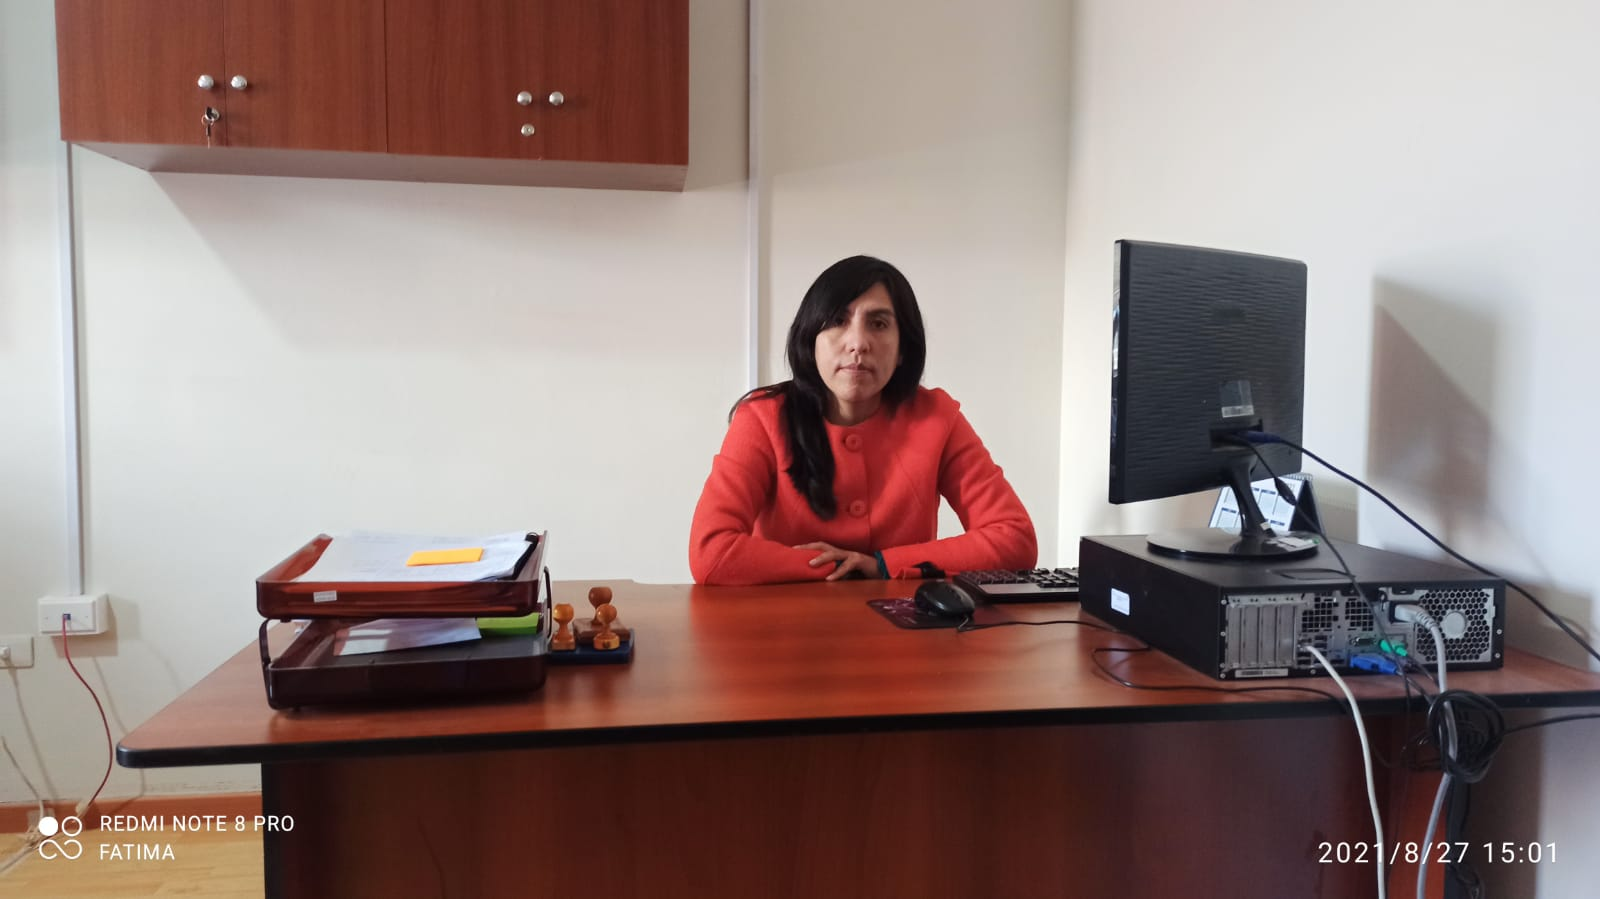
\includegraphics[width=8.5cm]{../editorial/foto_editorial.jpeg}
		\caption*{
			\centering
				MSC. Fátima Rosario Concha Velasco
				
				\textit{Directora de Epidemiología e Investigación}
				
				GERESA, Cusco }
	\end{wrapfigure}
	
	\noindent Un nuevo coronavirus, el SARS-CoV-2, apareció en diciembre del 2019, cuya transmisión a través del contacto directo o gotitas respiratorias dependiendo del tiempo y contacto cercano es más fácil y rápida en relación a los otros coronovarius. El virus se propagó rápidamente por todo el mundo a través de los viajeros, generando a la vez un incremento de la mortalidad. Se reconoce que los números notificados son subestimaciones de los casos de infección reales, considerando a los individuos asintomáticos con COVID-19 que no fueron identificados y rastreados.
	A nivel mundial, los gobiernos y las agencias tomaron medidas para contener la propagación de COVID-19, con rutinas aplicadas para la atención sanitaria y el distanciamiento social. Aun así, estas estrategias tuvieron consecuencias, como la crisis económica por el cierre de negocios y el cese de labores en diversas industrias. La calidad de la educación se vio afectada, ya que muchas escuelas carecían de plataformas y servicios de red. Por lo cual, la necesidad de continuar con la reactivación económica, traduce fortalecer a la brevedad la vacunación para COVID-19 en todos los grupos etarios. Continuar con las recomendaciones comunitarias para el distanciamiento y uso de máscaras que incluyen la prevención combinada y control de la fuente para las personas sintomáticas y asintomáticas. Así como, continuar con la oportuna identificación y rastreo de contactos de sintomáticos y asintomáticos.
	La vacunación preventiva generalizada puede reducir costos y desempeñar un papel fundamental en la protección de las personas contra la infección por COVID-19, facilitando la reducción significativa de la transmisión dentro de la población del rebaño. La preocupación de depender de las vacunas “sólo S”, por la presencia de mutaciones en la proteína pico (S) del SARS-CoV-2, genera una selección de variantes de COVID-19, con la ausencia del anticuerpo del huésped para empujar sistemáticamente al virus en una dirección determinada, aumentando la transmisibilidad y competencia entre ellas que podrían afectar la neutralización por sueros convalecientes. Siendo necesario considerar tanto la magnitud del cambio en la neutralización de anticuerpos, así como la posibilidad de que muchas vacunas candidatas necesiten ser rediseñadas y probadas.  Sin embargo, hasta la fecha, la vacunación para COVID-19 aun es la mejor manera de combatir la infección por SARS-CoV-2. Se han aprobado 8 tipos de vacuna para ser aplicados entre grupos prioritarios bajo una autorización de uso de emergencia (EUA), incluida la vacuna Moderna mRNA-1273, vacuna Pfizer-BioNtech BNT162b2, China Las vacunas CoronaVac ™ y COVID-19 de Sinopharm, las vacunas Sputnik V y EpiVacCorona de Rusia, el nuevo coronavirus ChAdOx1 2019 de AstraZeneca (nCoV-19), y el Ad26.COV2.S. de Janssen.
	Por lo cual, a partir del conocimiento generado en la información de la situación actual de COVID-19 en la Región Cusco, es importante continuar fortaleciendo la vacunación para COVID-19, la cual como se ha mencionado es la principal herramienta en la lucha contra el COVID-19, ayudándonos a desarrollar inmunidad, protegiendo a las personas que nos rodean, principalmente a los que tienen más riesgo de complicaciones graves. Así como también, es necesario que se siga fortaleciendo la detección y rastreo oportuno de casos para facilitar el control de la transmisión de la enfermedad.
	

	
	\begin{figure}[h]
		\caption{Tendencia Provincial de Incidencia acumulada de COVID-19, hasta la SE 38, 2021}\label{fig:mortalidad_provincias}
		\begin{center}
			\includegraphics[width=0.65\linewidth]{../figuras/figura17}
		\end{center}
		{\footnotesize {Fuente de datos: SINADEF.}}
	\end{figure}
	
	\newpage
	
	\section*{Evaluación Provincial de 5 Indicadores}
	\noindent El objetivo de estas figuras es comparar a cada provincia consigo misma de acuerdo a su historia  en la primera ola (en el año 2020). Se evaluaron los siguientes indicadores: incidencia, tasa de mortalidad, tasa de positividad molecular, tasa de positividad antigénica, y exceso de defunciones para cada provincia.
	
	\subsection*{Provincia de Acomayo}
	\noindent Las figuras inferiores (Figura \ref{fig:inc_mort_acomayo}, \ref{fig:positividad_acomayo}) muestran una importante disminución de la mortalidad e incidencia en estas últimas semanas, siendo mayor a partir de la SE 20. La tasa de positividad molecular y antigénica disminuyeron en las últimas semanas. En la Figura \ref{fig:exceso_acomayo} se muestra que no hay exceso de defunciones respecto al año 2019.
	
	\begin{figure}[h]
		\caption{Tasa de Incidencia y Mortalidad Comparativa en la Provincia de Acomayo 2020 y 2021, hasta la SE 38}\label{fig:inc_mort_acomayo}
		\begin{center}
			\includegraphics[width=0.7\linewidth]{../figuras/provincia_m1}
		\end{center}
		{\footnotesize {Fuente de datos: NOTICOVID, SISCOVID, SINADEF.}}
	\end{figure}

	\begin{figure}[h]
	\caption{Tasa de Positividad de Prueba Molecular y Antigénica Comparativa en la Provincia de Acomayo 2020 y 2021, hasta la SE 38}\label{fig:positividad_acomayo}
	\begin{center}
		\includegraphics[width=0.7\linewidth]{../figuras/provincia_p1}
	\end{center}
	{\footnotesize {Fuente de datos: NOTICOVID, SISCOVID.}}
	\end{figure}

	\begin{figure}[h]
	\caption{Exceso de Defunciones Comparativo en la Provincia de Acomayo 2019, 2020 y 2021, hasta la SE 38}\label{fig:exceso_acomayo}
	\begin{center}
		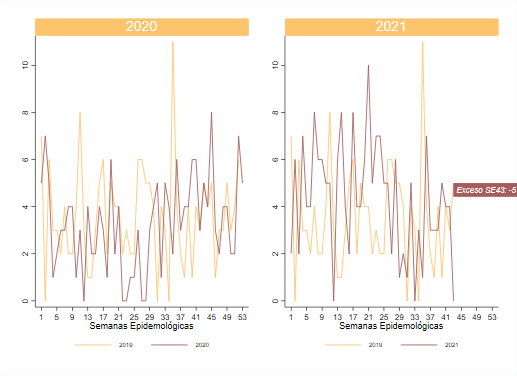
\includegraphics[width=0.7\linewidth]{../figuras/exceso_1}
	\end{center}
	{\footnotesize {Fuente de datos: SINADEF.}}
	\end{figure}

	% Anta
	\clearpage
	
	\subsection*{Provincia de Anta}
	\noindent Las figuras de abajo (Figura \ref{fig:inc_mort_anta}, \ref{fig:positividad_anta})  muestran una disminución importante desde la SE13 en la tasa de mortalidad, que aunque aumentó desde la SE33, llegó a ser bastante baja en la SE38. Similarmente, la tasa de incidencia tiene una caída más sostenida. Hay un pequeño aumento en la tasa de positividad de pruebas moleculares similar a la de pruebas antigénicas estas últimas semanas. En la Figura \ref{fig:exceso_anta} se muestra que no hay exceso de defunciones respecto al año 2019.
	
		\begin{figure}[h]
		\caption{Tasa de Incidencia y Mortalidad Comparativa en la Provincia de Anta 2020 y 2021, hasta la SE 38}\label{fig:inc_mort_anta}
		\begin{center}
			\includegraphics[width=0.7\linewidth]{../figuras/provincia_m2}
		\end{center}
		{\footnotesize {Fuente de datos: NOTICOVID, SISCOVID, SINADEF.}}
	\end{figure}
	
	\begin{figure}[h]
		\caption{Tasa de Positividad de Prueba Molecular y Antigénica Comparativa en la Provincia de Anta 2020 y 2021, hasta la SE 38}\label{fig:positividad_anta}
		\begin{center}
			\includegraphics[width=0.7\linewidth]{../figuras/provincia_p2}
		\end{center}
		{\footnotesize {Fuente de datos: NOTICOVID, SISCOVID.}}
	\end{figure}
	
	\begin{figure}[h]
		\caption{Exceso de Defunciones Comparativo en la Provincia de Anta 2019, 2020 y 2021, hasta la SE 38}\label{fig:exceso_anta}
		\begin{center}
			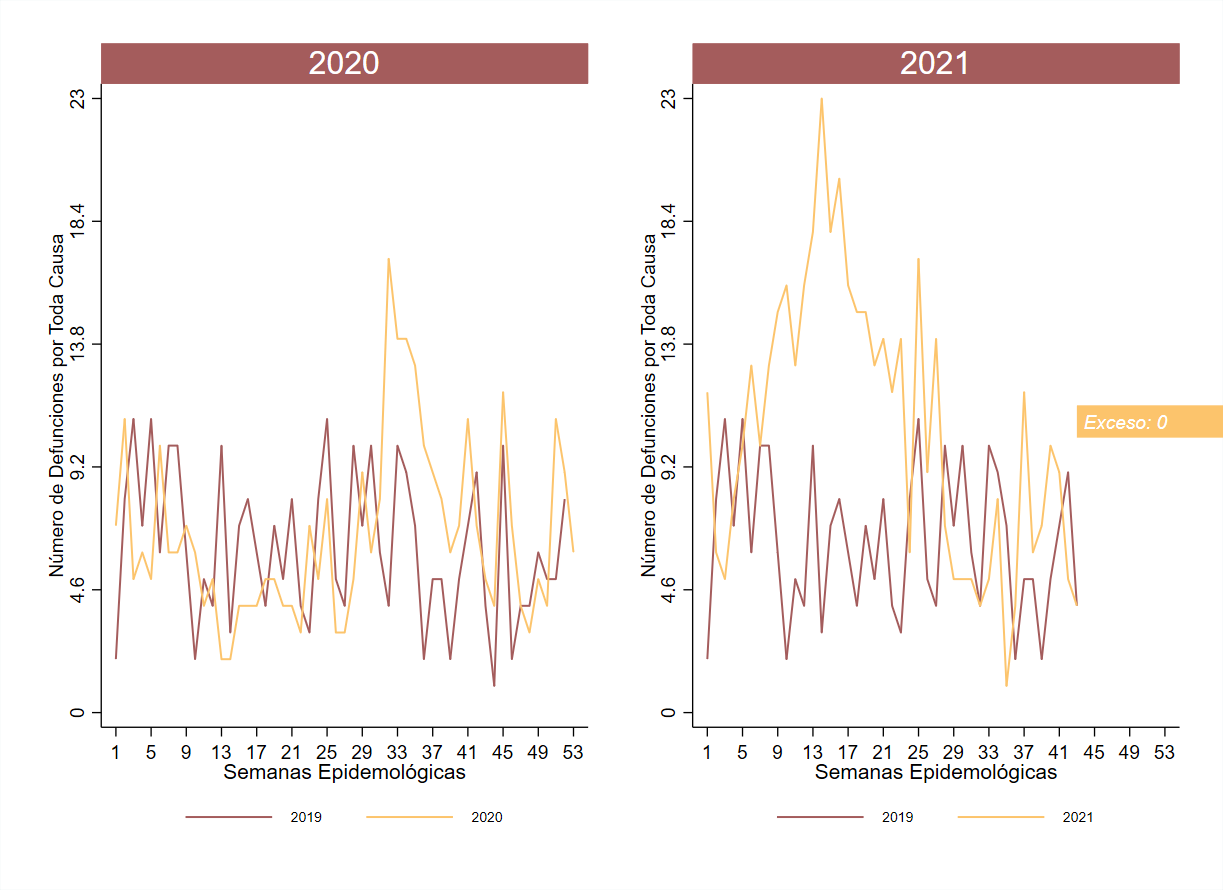
\includegraphics[width=0.7\linewidth]{../figuras/exceso_2}
		\end{center}
		{\footnotesize {Fuente de datos: SINADEF.}}
	\end{figure}

	% Canas
		\clearpage
	
	\subsection*{Provincia de Canas}
	\noindent Las figuras de abajo (Figura \ref{fig:inc_mort_canas}, \ref{fig:positividad_canas})  muestran una disminución importante desde la SE13 en la tasa de mortalidad, que aunque aumentó desde la SE33, llegó a ser bastante baja en la SE38. Similarmente, la tasa de incidencia tiene una caída más sostenida. Hay un pequeño aumento en la tasa de positividad de pruebas moleculares similar a la de pruebas antigénicas estas últimas semanas. En la Figura \ref{fig:exceso_canas} se muestra que no hay exceso de defunciones respecto al año 2019.
	
	\begin{figure}[h]
		\caption{Tasa de Incidencia y Mortalidad Comparativa en la Provincia de Canas 2020 y 2021, hasta la SE 38}\label{fig:inc_mort_canas}
		\begin{center}
			\includegraphics[width=0.7\linewidth]{../figuras/provincia_m3}
		\end{center}
		{\footnotesize {Fuente de datos: NOTICOVID, SISCOVID, SINADEF.}}
	\end{figure}
	
	\begin{figure}[h]
		\caption{Tasa de Positividad de Prueba Molecular y Antigénica Comparativa en la Provincia de Canas 2020 y 2021, hasta la SE 38}\label{fig:positividad_canas}
		\begin{center}
			\includegraphics[width=0.7\linewidth]{../figuras/provincia_p3}
		\end{center}
		{\footnotesize {Fuente de datos: NOTICOVID, SISCOVID.}}
	\end{figure}
	
	\begin{figure}[h]
		\caption{Exceso de Defunciones Comparativo en la Provincia de Canas 2019, 2020 y 2021, hasta la SE 38}\label{fig:exceso_canas}
		\begin{center}
			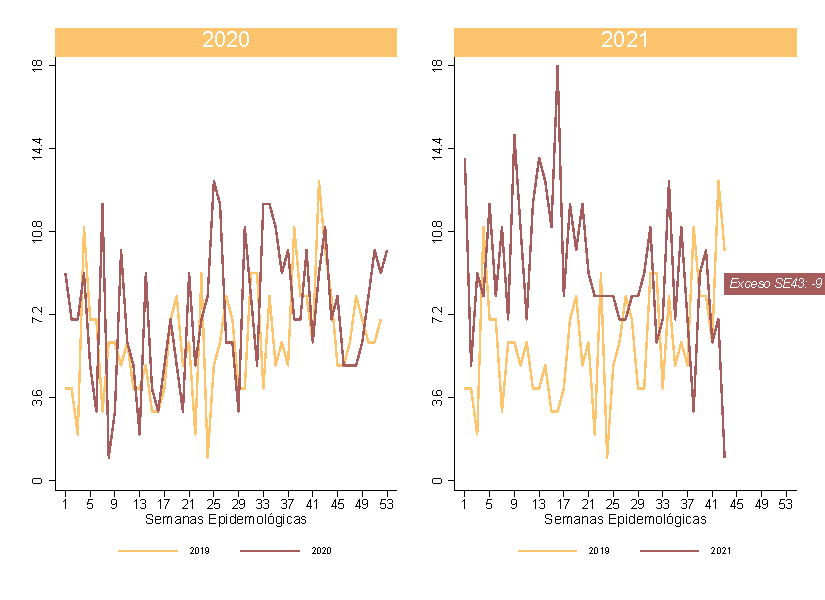
\includegraphics[width=0.7\linewidth]{../figuras/exceso_3}
		\end{center}
		{\footnotesize {Fuente de datos: SINADEF.}}
	\end{figure}

	% Calca
\clearpage

	\subsection*{Provincia de Calca}
	\noindent Las figuras de abajo (Figura \ref{fig:inc_mort_calca}, \ref{fig:positividad_calca})  muestran una disminución importante desde la SE13 en la tasa de mortalidad, que aunque aumentó desde la SE33, llegó a ser bastante baja en la SE38. Similarmente, la tasa de incidencia tiene una caída más sostenida. Hay un pequeño aumento en la tasa de positividad de pruebas moleculares similar a la de pruebas antigénicas estas últimas semanas. En la Figura \ref{fig:exceso_calca} se muestra que no hay exceso de defunciones respecto al año 2019.

	\begin{figure}[h]
	\caption{Tasa de Incidencia y Mortalidad Comparativa en la Provincia de Canas 2020 y 2021, hasta la SE 38}\label{fig:inc_mort_calca}
	\begin{center}
		\includegraphics[width=0.7\linewidth]{../figuras/provincia_m4}
	\end{center}
	{\footnotesize {Fuente de datos: NOTICOVID, SISCOVID, SINADEF.}}
	\end{figure}

	\begin{figure}[h]
	\caption{Tasa de Positividad de Prueba Molecular y Antigénica Comparativa en la Provincia de Canas 2020 y 2021, hasta la SE 38}\label{fig:positividad_calca}
	\begin{center}
		\includegraphics[width=0.7\linewidth]{../figuras/provincia_p4}
	\end{center}
	{\footnotesize {Fuente de datos: NOTICOVID, SISCOVID.}}
	\end{figure}

	\begin{figure}[h]
	\caption{Exceso de Defunciones Comparativo en la Provincia de Canas 2019, 2020 y 2021, hasta la SE 38}\label{fig:exceso_calca}
	\begin{center}
		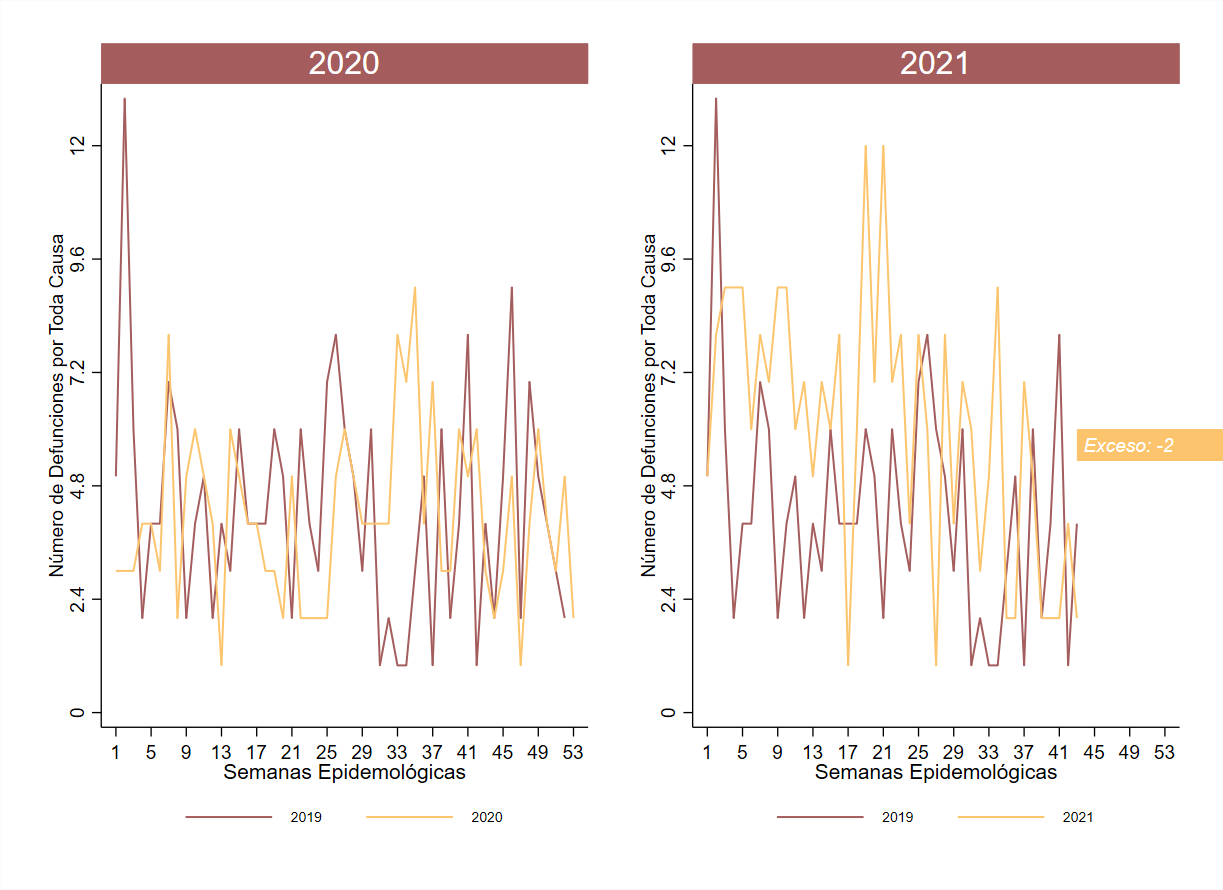
\includegraphics[width=0.7\linewidth]{../figuras/exceso_4}
	\end{center}
	{\footnotesize {Fuente de datos: SINADEF.}}
	\end{figure}

	% Canas
\clearpage

	\subsection*{Provincia de Canchis}
	\noindent Las figuras de abajo (Figura \ref{fig:inc_mort_canchis}, \ref{fig:positividad_canchis})  muestran una disminución importante desde la SE13 en la tasa de mortalidad, que aunque aumentó desde la SE33, llegó a ser bastante baja en la SE38. Similarmente, la tasa de incidencia tiene una caída más sostenida. Hay un pequeño aumento en la tasa de positividad de pruebas moleculares similar a la de pruebas antigénicas estas últimas semanas. En la Figura \ref{fig:exceso_canchis} se muestra que no hay exceso de defunciones respecto al año 2019.

	\begin{figure}[h]
	\caption{Tasa de Incidencia y Mortalidad Comparativa en la Provincia de Canas 2020 y 2021, hasta la SE 38}\label{fig:inc_mort_canchis}
	\begin{center}
		\includegraphics[width=0.7\linewidth]{../figuras/provincia_m5}
	\end{center}
	{\footnotesize {Fuente de datos: NOTICOVID, SISCOVID, SINADEF.}}
	\end{figure}

	\begin{figure}[h]
	\caption{Tasa de Positividad de Prueba Molecular y Antigénica Comparativa en la Provincia de Canas 2020 y 2021, hasta la SE 38}\label{fig:positividad_canchis}
	\begin{center}
		\includegraphics[width=0.7\linewidth]{../figuras/provincia_p5}
	\end{center}
	{\footnotesize {Fuente de datos: NOTICOVID, SISCOVID.}}
	\end{figure}
	
	\begin{figure}[h]
	\caption{Exceso de Defunciones Comparativo en la Provincia de Canas 2019, 2020 y 2021, hasta la SE 38}\label{fig:exceso_canchis}
	\begin{center}
		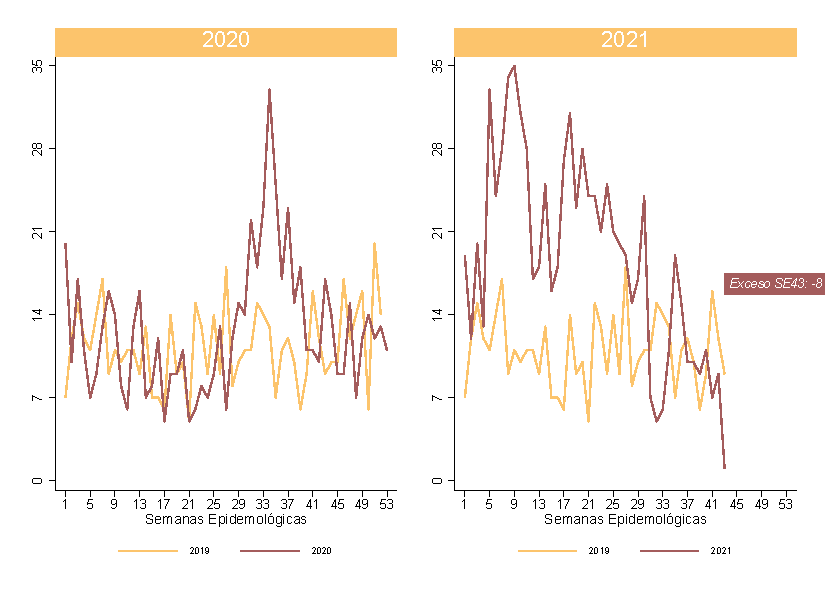
\includegraphics[width=0.7\linewidth]{../figuras/exceso_5}
	\end{center}
	{\footnotesize {Fuente de datos: SINADEF.}}
	\end{figure}

\clearpage

	% Chumbivilcas
	\subsection*{Provincia de Chumbivilcas}
	\noindent Las figuras de abajo (Figura \ref{fig:inc_mort_chumbivilcas}, \ref{fig:positividad_chumbivilcas})  muestran una disminución importante desde la SE13 en la tasa de mortalidad, que aunque aumentó desde la SE33, llegó a ser bastante baja en la SE38. Similarmente, la tasa de incidencia tiene una caída más sostenida. Hay un pequeño aumento en la tasa de positividad de pruebas moleculares similar a la de pruebas antigénicas estas últimas semanas. En la Figura \ref{fig:exceso_chumbivilcas} se muestra que no hay exceso de defunciones respecto al año 2019.

	\begin{figure}[h]
	\caption{Tasa de Incidencia y Mortalidad Comparativa en la Provincia de Chumbivilcas 2020 y 2021, hasta la SE 38}\label{fig:inc_mort_chumbivilcas}
	\begin{center}
		\includegraphics[width=0.7\linewidth]{../figuras/provincia_m6}
	\end{center}
	{\footnotesize {Fuente de datos: NOTICOVID, SISCOVID, SINADEF.}}
	\end{figure}

	\begin{figure}[h]
	\caption{Tasa de Positividad de Prueba Molecular y Antigénica Comparativa en la Provincia de Chumbivilcas 2020 y 2021, hasta la SE 38}\label{fig:positividad_chumbivilcas}
	\begin{center}
		\includegraphics[width=0.7\linewidth]{../figuras/provincia_p6}
	\end{center}
	{\footnotesize {Fuente de datos: NOTICOVID, SISCOVID.}}
	\end{figure}

	\begin{figure}[h]
	\caption{Exceso de Defunciones Comparativo en la Provincia de Chumbivilcas 2019, 2020 y 2021, hasta la SE 38}\label{fig:exceso_chumbivilcas}
	\begin{center}
		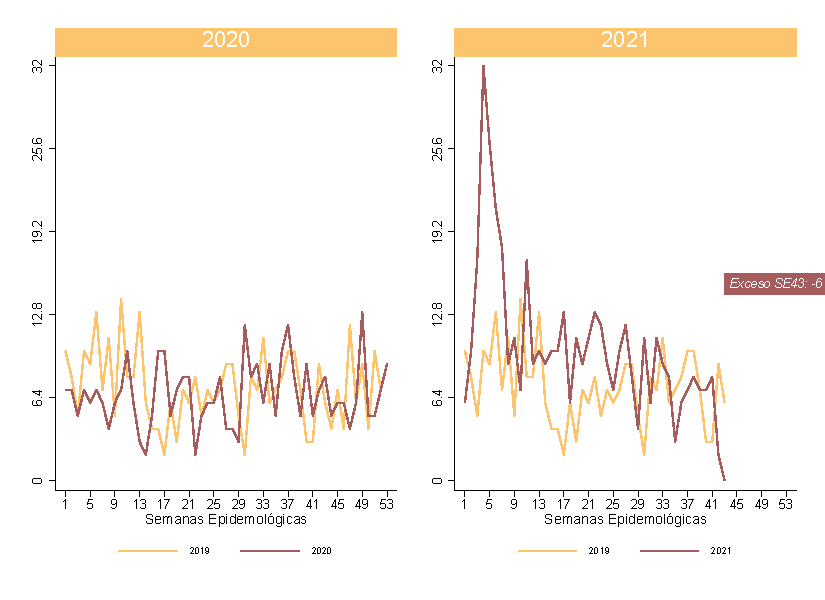
\includegraphics[width=0.7\linewidth]{../figuras/exceso_6}
	\end{center}
	{\footnotesize {Fuente de datos: SINADEF.}}
	\end{figure}

% Cusco
\clearpage

	\subsection*{Provincia de Cusco}
	\noindent Las figuras de abajo (Figura \ref{fig:inc_mort_cusco}, \ref{fig:positividad_cusco})  muestran una disminución importante desde la SE13 en la tasa de mortalidad, que aunque aumentó desde la SE33, llegó a ser bastante baja en la SE38. Similarmente, la tasa de incidencia tiene una caída más sostenida. Hay un pequeño aumento en la tasa de positividad de pruebas moleculares similar a la de pruebas antigénicas estas últimas semanas. En la Figura \ref{fig:exceso_cusco} se muestra que no hay exceso de defunciones respecto al año 2019.

	\begin{figure}[h]
	\caption{Tasa de Incidencia y Mortalidad Comparativa en la Provincia de Cusco 2020 y 2021, hasta la SE 38}\label{fig:inc_mort_cusco}
	\begin{center}
		\includegraphics[width=0.7\linewidth]{../figuras/provincia_m7}
	\end{center}
	{\footnotesize {Fuente de datos: NOTICOVID, SISCOVID, SINADEF.}}
	\end{figure}

	\begin{figure}[h]
	\caption{Tasa de Positividad de Prueba Molecular y Antigénica Comparativa en la Provincia de Cusco 2020 y 2021, hasta la SE 38}\label{fig:positividad_cusco}
	\begin{center}
		\includegraphics[width=0.7\linewidth]{../figuras/provincia_p7}
	\end{center}
	{\footnotesize {Fuente de datos: NOTICOVID, SISCOVID.}}
	\end{figure}

	\begin{figure}[h]
	\caption{Exceso de Defunciones Comparativo en la Provincia de Cusco 2019, 2020 y 2021, hasta la SE 38}\label{fig:exceso_cusco}
	\begin{center}
		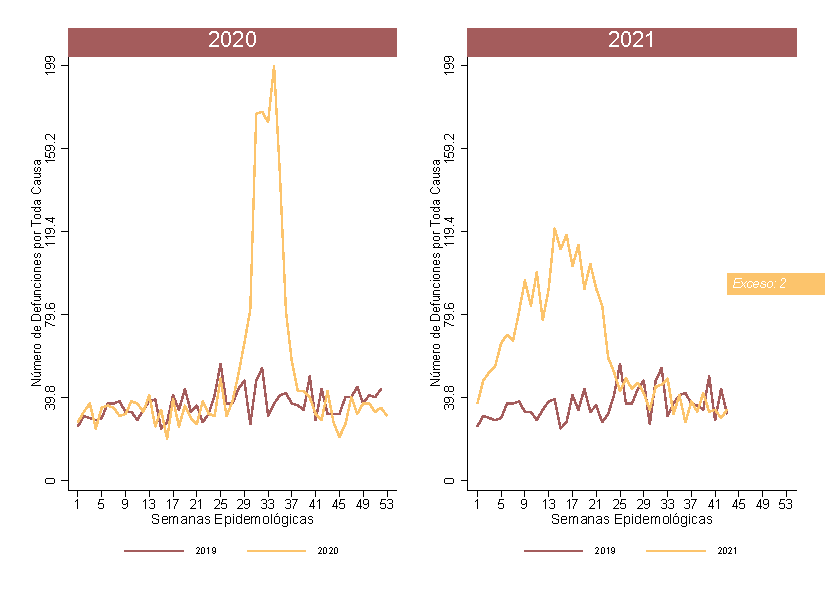
\includegraphics[width=0.7\linewidth]{../figuras/exceso_7}
	\end{center}
	{\footnotesize {Fuente de datos: SINADEF.}}
	\end{figure}

% Espinar
\clearpage

	\subsection*{Provincia de Espinar}
	\noindent Las figuras de abajo (Figura \ref{fig:inc_mort_espinar}, \ref{fig:positividad_espinar})  muestran una disminución importante desde la SE13 en la tasa de mortalidad, que aunque aumentó desde la SE33, llegó a ser bastante baja en la SE38. Similarmente, la tasa de incidencia tiene una caída más sostenida. Hay un pequeño aumento en la tasa de positividad de pruebas moleculares similar a la de pruebas antigénicas estas últimas semanas. En la Figura \ref{fig:exceso_espinar} se muestra que no hay exceso de defunciones respecto al año 2019.

	\begin{figure}[h]
	\caption{Tasa de Incidencia y Mortalidad Comparativa en la Provincia de Espinar 2020 y 2021, hasta la SE 38}\label{fig:inc_mort_espinar}
	\begin{center}
		\includegraphics[width=0.7\linewidth]{../figuras/provincia_m8}
	\end{center}
	{\footnotesize {Fuente de datos: NOTICOVID, SISCOVID, SINADEF.}}
	\end{figure}

	\begin{figure}[h]
	\caption{Tasa de Positividad de Prueba Molecular y Antigénica Comparativa en la Provincia de Espinar 2020 y 2021, hasta la SE 38}\label{fig:positividad_espinar}
	\begin{center}
		\includegraphics[width=0.7\linewidth]{../figuras/provincia_p8}
	\end{center}
	{\footnotesize {Fuente de datos: NOTICOVID, SISCOVID.}}
	\end{figure}

	\begin{figure}[h]
	\caption{Exceso de Defunciones Comparativo en la Provincia de Espinar 2019, 2020 y 2021, hasta la SE 38}\label{fig:exceso_espinar}
	\begin{center}
		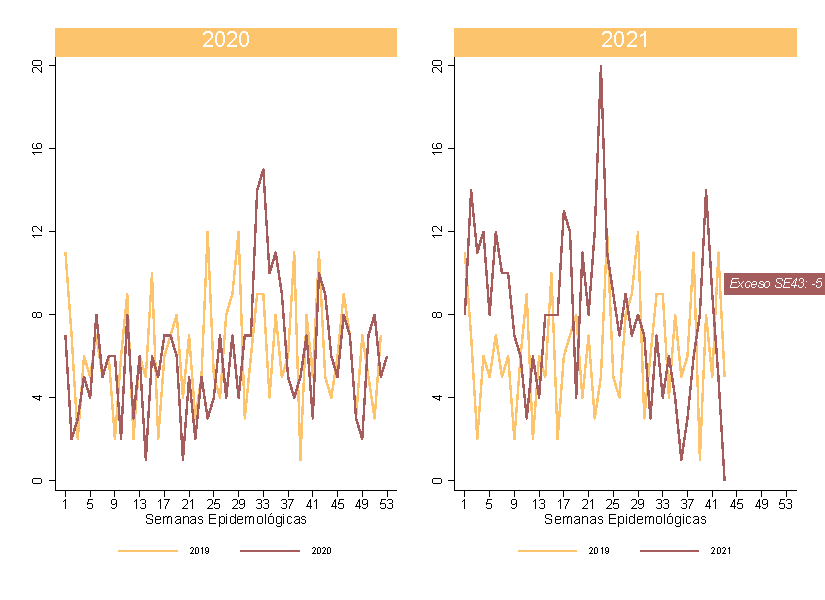
\includegraphics[width=0.7\linewidth]{../figuras/exceso_8}
	\end{center}
	{\footnotesize {Fuente de datos: SINADEF.}}
	\end{figure}

% La Convención
\clearpage

	\subsection*{Provincia de La Convención}
	\noindent Las figuras de abajo (Figura \ref{fig:inc_mort_laconv}, \ref{fig:positividad_laconv})  muestran una disminución importante desde la SE13 en la tasa de mortalidad, que aunque aumentó desde la SE33, llegó a ser bastante baja en la SE38. Similarmente, la tasa de incidencia tiene una caída más sostenida. Hay un pequeño aumento en la tasa de positividad de pruebas moleculares similar a la de pruebas antigénicas estas últimas semanas. En la Figura \ref{fig:exceso_laconv} se muestra que no hay exceso de defunciones respecto al año 2019.

	\begin{figure}[h]
	\caption{Tasa de Incidencia y Mortalidad Comparativa en la Provincia de La Convención 2020 y 2021, hasta la SE 38}\label{fig:inc_mort_laconv}
	\begin{center}
		\includegraphics[width=0.7\linewidth]{../figuras/provincia_m9}
	\end{center}
	{\footnotesize {Fuente de datos: NOTICOVID, SISCOVID, SINADEF.}}
	\end{figure}

	\begin{figure}[h]
	\caption{Tasa de Positividad de Prueba Molecular y Antigénica Comparativa en la Provincia de La Convención 2020 y 2021, hasta la SE 38}\label{fig:positividad_laconv}
	\begin{center}
		\includegraphics[width=0.7\linewidth]{../figuras/provincia_p9}
	\end{center}
	{\footnotesize {Fuente de datos: NOTICOVID, SISCOVID.}}
	\end{figure}

	\begin{figure}[h]
	\caption{Exceso de Defunciones Comparativo en la Provincia de La Convención 2019, 2020 y 2021, hasta la SE 38}\label{fig:exceso_laconv}
	\begin{center}
		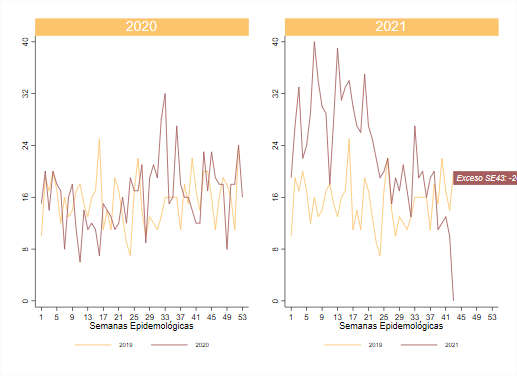
\includegraphics[width=0.7\linewidth]{../figuras/exceso_9}
	\end{center}
	{\footnotesize {Fuente de datos: SINADEF.}}
	\end{figure}

% Paruro
\clearpage

	\subsection*{Provincia de Paruro}
	\noindent Las figuras de abajo (Figura \ref{fig:inc_mort_paruro}, \ref{fig:positividad_paruro})  muestran una disminución importante desde la SE13 en la tasa de mortalidad, que aunque aumentó desde la SE33, llegó a ser bastante baja en la SE38. Similarmente, la tasa de incidencia tiene una caída más sostenida. Hay un pequeño aumento en la tasa de positividad de pruebas moleculares similar a la de pruebas antigénicas estas últimas semanas. En la Figura \ref{fig:exceso_paruro} se muestra que no hay exceso de defunciones respecto al año 2019.

	\begin{figure}[h]
	\caption{Tasa de Incidencia y Mortalidad Comparativa en la Provincia de Paruro 2020 y 2021, hasta la SE 38}\label{fig:inc_mort_paruro}
	\begin{center}
		\includegraphics[width=0.7\linewidth]{../figuras/provincia_m10}
	\end{center}
	{\footnotesize {Fuente de datos: NOTICOVID, SISCOVID, SINADEF.}}
	\end{figure}

	\begin{figure}[h]
	\caption{Tasa de Positividad de Prueba Molecular y Antigénica Comparativa en la Provincia de Paruro 2020 y 2021, hasta la SE 38}\label{fig:positividad_paruro}
	\begin{center}
		\includegraphics[width=0.7\linewidth]{../figuras/provincia_p10}
	\end{center}
	{\footnotesize {Fuente de datos: NOTICOVID, SISCOVID.}}
	\end{figure}

	\begin{figure}[h]
	\caption{Exceso de Defunciones Comparativo en la Provincia de Paruro 2019, 2020 y 2021, hasta la SE 38}\label{fig:exceso_paruro}
	\begin{center}
		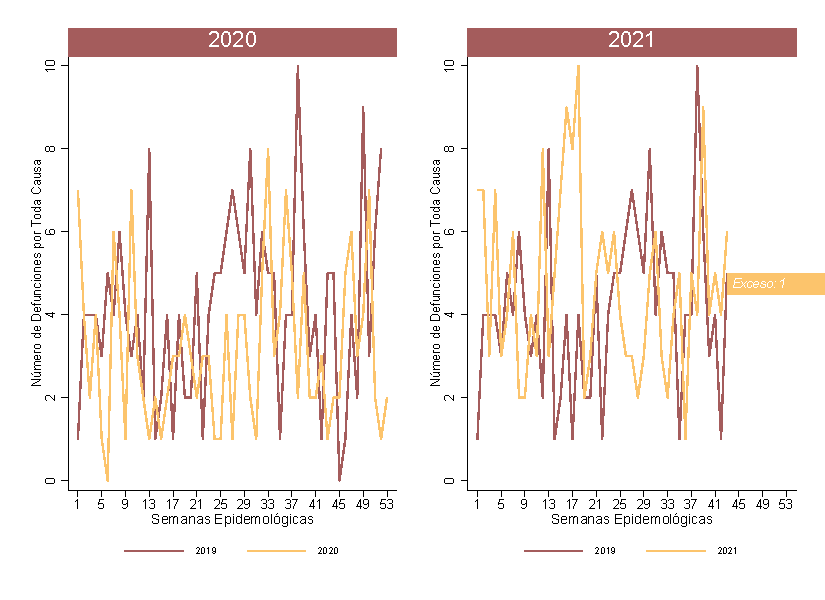
\includegraphics[width=0.7\linewidth]{../figuras/exceso_10}
	\end{center}
	{\footnotesize {Fuente de datos: SINADEF.}}
	\end{figure}


% Paucartambo
\clearpage

	\subsection*{Provincia de Paucartambo}
	\noindent Las figuras de abajo (Figura \ref{fig:inc_mort_paucartam}, \ref{fig:positividad_paucartam})  muestran una disminución importante desde la SE13 en la tasa de mortalidad, que aunque aumentó desde la SE33, llegó a ser bastante baja en la SE38. Similarmente, la tasa de incidencia tiene una caída más sostenida. Hay un pequeño aumento en la tasa de positividad de pruebas moleculares similar a la de pruebas antigénicas estas últimas semanas. En la Figura \ref{fig:exceso_paucartam} se muestra que no hay exceso de defunciones respecto al año 2019.

	\begin{figure}[h]
	\caption{Tasa de Incidencia y Mortalidad Comparativa en la Provincia de Paucartambo 2020 y 2021, hasta la SE 38}\label{fig:inc_mort_paucartam}
	\begin{center}
		\includegraphics[width=0.7\linewidth]{../figuras/provincia_m11}
	\end{center}
	{\footnotesize {Fuente de datos: NOTICOVID, SISCOVID, SINADEF.}}
	\end{figure}

	\begin{figure}[h]
	\caption{Tasa de Positividad de Prueba Molecular y Antigénica Comparativa en la Provincia de Paucartambo 2020 y 2021, hasta la SE 38}\label{fig:positividad_paucartam}
	\begin{center}
		\includegraphics[width=0.7\linewidth]{../figuras/provincia_p11}
	\end{center}
	{\footnotesize {Fuente de datos: NOTICOVID, SISCOVID.}}
	\end{figure}

	\begin{figure}[h]
	\caption{Exceso de Defunciones Comparativo en la Provincia de Paucartambo 2019, 2020 y 2021, hasta la SE 38}\label{fig:exceso_paucartam}
	\begin{center}
		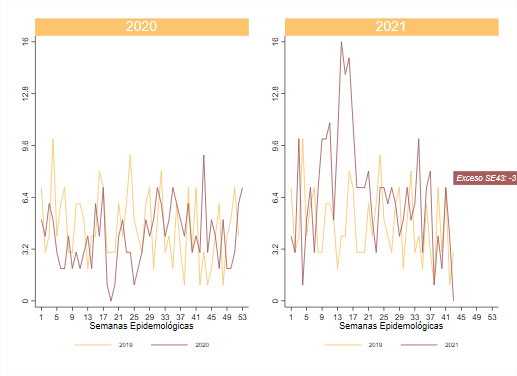
\includegraphics[width=0.7\linewidth]{../figuras/exceso_11}
	\end{center}
	{\footnotesize {Fuente de datos: SINADEF.}}
	\end{figure}

% Quispicanchi
\clearpage

	\subsection*{Provincia de Quispicanchi}
	\noindent Las figuras de abajo (Figura \ref{fig:inc_mort_quisp}, \ref{fig:positividad_quisp})  muestran una disminución importante desde la SE13 en la tasa de mortalidad, que aunque aumentó desde la SE33, llegó a ser bastante baja en la SE38. Similarmente, la tasa de incidencia tiene una caída más sostenida. Hay un pequeño aumento en la tasa de positividad de pruebas moleculares similar a la de pruebas antigénicas estas últimas semanas. En la Figura \ref{fig:exceso_quisp} se muestra que no hay exceso de defunciones respecto al año 2019.

	\begin{figure}[h]
	\caption{Tasa de Incidencia y Mortalidad Comparativa en la Provincia de Quispicanchi 2020 y 2021, hasta la SE 38}\label{fig:inc_mort_quisp}
	\begin{center}
		\includegraphics[width=0.7\linewidth]{../figuras/provincia_m12}
	\end{center}
	{\footnotesize {Fuente de datos: NOTICOVID, SISCOVID, SINADEF.}}
	\end{figure}

	\begin{figure}[h]
	\caption{Tasa de Positividad de Prueba Molecular y Antigénica Comparativa en la Provincia de Quispicanchi 2020 y 2021, hasta la SE 38}\label{fig:positividad_quisp}
	\begin{center}
		\includegraphics[width=0.7\linewidth]{../figuras/provincia_p12}
	\end{center}
	{\footnotesize {Fuente de datos: NOTICOVID, SISCOVID.}}
	\end{figure}

	\begin{figure}[h]
	\caption{Exceso de Defunciones Comparativo en la Provincia de Quispicanchi 2019, 2020 y 2021, hasta la SE 38}\label{fig:exceso_quisp}
	\begin{center}
		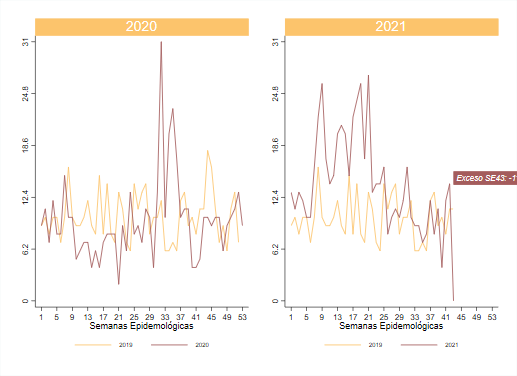
\includegraphics[width=0.7\linewidth]{../figuras/exceso_12}
	\end{center}
	{\footnotesize {Fuente de datos: SINADEF.}}
	\end{figure}

% Urubamba
\clearpage

	\subsection*{Provincia de Urubamba}
	\noindent Las figuras de abajo (Figura \ref{fig:inc_urub}, \ref{fig:positividad_urub})  muestran una disminución importante desde la SE13 en la tasa de mortalidad, que aunque aumentó desde la SE33, llegó a ser bastante baja en la SE38. Similarmente, la tasa de incidencia tiene una caída más sostenida. Hay un pequeño aumento en la tasa de positividad de pruebas moleculares similar a la de pruebas antigénicas estas últimas semanas. En la Figura \ref{fig:exceso_urub} se muestra que no hay exceso de defunciones respecto al año 2019.

	\begin{figure}[h]
	\caption{Tasa de Incidencia y Mortalidad Comparativa en la Provincia de Urubamba 2020 y 2021, hasta la SE 38}\label{fig:inc_urub}
	\begin{center}
		\includegraphics[width=0.7\linewidth]{../figuras/provincia_m13}
	\end{center}
	{\footnotesize {Fuente de datos: NOTICOVID, SISCOVID, SINADEF.}}
	\end{figure}

	\begin{figure}[h]
	\caption{Tasa de Positividad de Prueba Molecular y Antigénica Comparativa en la Provincia de Urubamba 2020 y 2021, hasta la SE 38}\label{fig:positividad_urub}
	\begin{center}
		\includegraphics[width=0.7\linewidth]{../figuras/provincia_p13}
	\end{center}
	{\footnotesize {Fuente de datos: NOTICOVID, SISCOVID.}}
	\end{figure}

	\begin{figure}[h]
	\caption{Exceso de Defunciones Comparativo en la Provincia de Urubamba 2019, 2020 y 2021, hasta la SE 38}\label{fig:exceso_urub}
	\begin{center}
		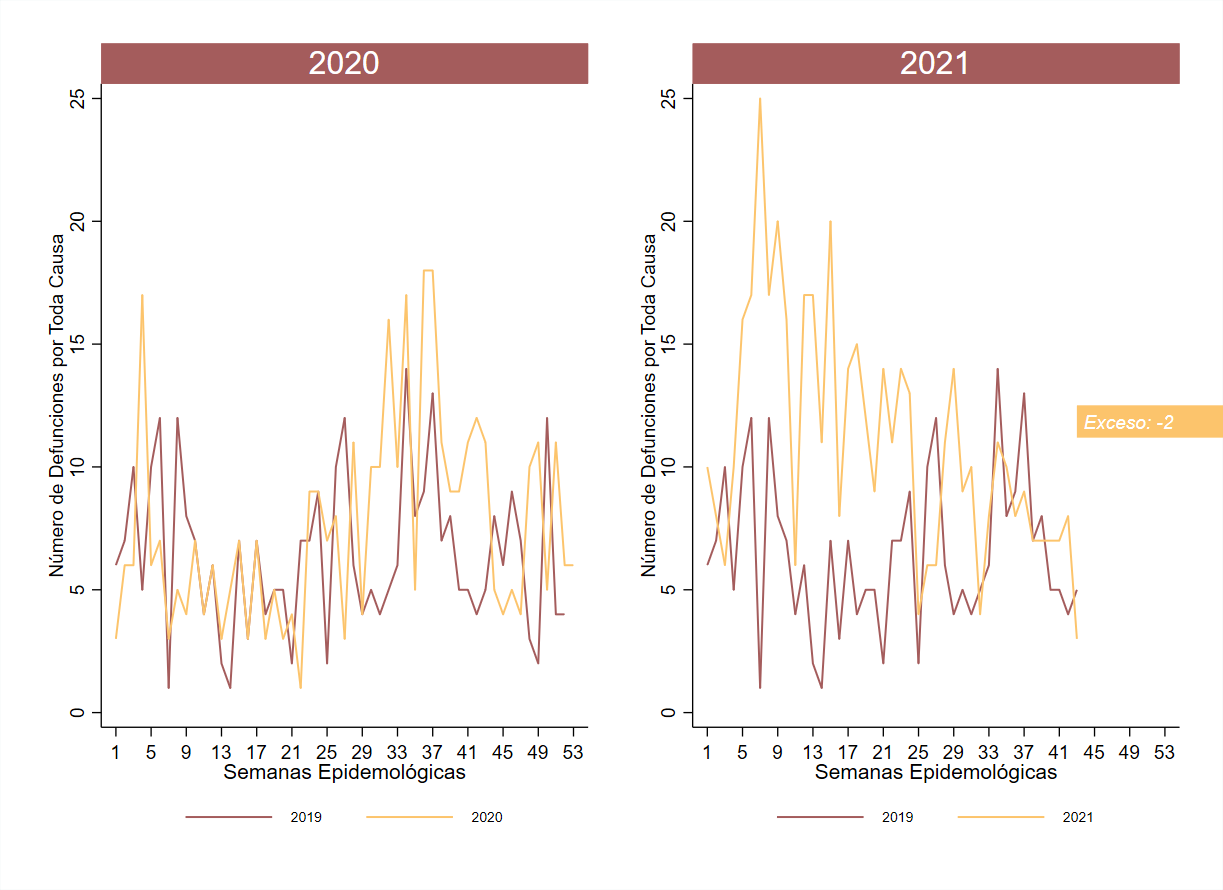
\includegraphics[width=0.7\linewidth]{../figuras/exceso_13}
	\end{center}
	{\footnotesize {Fuente de datos: SINADEF.}}
	\end{figure}
%---------------------------------------------------------------------------
% CAPÍTULO: VARIANTES DE COVID-19
%---------------------------------------------------------------------------
	\chapter*{Variantes de COVID-19}
	\addcontentsline{toc}{chapter}{Variantes de COVID-19}
	\noindent Las variantes genéticas del SARS-CoV-2 han estado emergiendo y circulando por el mundo durante toda la pandemia del COVID-19. Las variantes y mutaciones virales en la región Cusco son monitoreadas de forma rutinaria mediante la vigilancia secuencial realizada por el laboratorio referencial del Instituto Nacional de Salud. Asimismo, hasta la fecha se ha tenido la colaboración de la Universidad Nacional de San Antonio Abad del Cusco y de la Universidad Peruana Cayetano Heredia, con las que se ha realizado investigaciones epidemiológicas de secuenciamiento viral en SARS-CoV-2.
	
	A nivel de la región Cusco hasta la SE 38,  se realizó el secuenciamiento genético a 262 pruebas positivas para COVID-19, en la Figura 31C se muestra el porcentaje (\%) de cada variante encontrada. Se observa que la variante más prevalente (78.49\%) corresponde a la variante Lambda, seguida de la variante gamma ( 13.44\%) y en menor proporción las variantes delta (B 1617), B1134 y B 1621.
	
	[Insertar figura]
	
%---------------------------------------------------------------------------
% CAPÍTULO: DEFUNCIONES CERO
%---------------------------------------------------------------------------
	\chapter*{Semanas con Cero Defunciones por COVID-19 por Semana a Nivel Provincial}
	\addcontentsline{toc}{chapter}{Defunciones Cero}
	\noindent En las últimas semanas ha existido un gran interés en la disminución de defunciones por COVID-19 a nivel nacional. Cusco ha experimentado una importante disminución de fallecidos por esta enfermedad.  La siguiente figura (Figura 32) muestra la cantidad de fallecidos por semana epidemiológica. Se muestra el análisis desde la semana 31 a la 38 (del 1 de agosto al 25 de septiembre). Las regiones pintadas de celeste indican cero fallecidos por COVID en la respectiva provincia.
	
	Es interesante notar que existe una disminución de defunciones en todas las provincias en el periodo analizado. Espinar es un caso notable en no reportar defunciones en estas últimas semanas. Aunque la Provincia Cusco siempre ha reportado fallecidos por COVID, ésta ha disminuido a lo largo del periodo analizado. La última semana (SE38) 9 de las 13 provincias reportaron cero defunciones.
	
	[Insertar figura]


%---------------------------------------------------------------------------
% CAPÍTULO: AGRADECIMIENTOS
%---------------------------------------------------------------------------
	\chapter*{Agradecimientos}
	\addcontentsline{toc}{chapter}{Agradecimientos}
		
	\centering
		{\large El presente Boletín Epidemiológico COVID-19 se ha elaborado gracias a la información y esfuerzo conjunto de los Equipos de Inteligencia Sanitaria de los Hospitales y Redes de la GERESA Cusco:

		\vspace{0.5cm}
		\noindent
		\begin{minipage}[t]{.45\textwidth}
			\centering
			Hospital Regional del Cusco \\
			M.S.P. Marina Ochoa Linares \vspace{0.5cm}\\
			Hospital Antonio Lorena \\
			Dr. Rony Monge \vspace{.5cm}\\
			Hospital Nacional Adolfo Guevara Velazco\\
			M.S.P. Lucio Velasquez Cuentas \vspace{.5cm}\\
			Red de Salud Norte \\
			M.C. Guido Giraldo Alencastre\vspace{0.5cm}\\
			Red de Salud Sur\\
			Lic. Luz Marina Bernable Villasante \vspace{0.5cm}\\	
		\end{minipage}
		\hfill
		\noindent
		\begin{minipage}[t]{.45\textwidth}
			\centering
			Red de Salud La Convención\\
			Dr. David Coanqui Pacori\vspace{0.5cm}\\
			Red de Salud Chumbivilcas\\
			Lic. Eduarda Benito Calderón \vspace{.5cm}\\
			Red de Salud Canas Canchis Espinar\\
			MC. William Achahui Mercado \vspace{.5cm}\\
			Red de Salud Kimbiri Pichari \\
			Lic Fiorela Alvarez Nihua\vspace{0.5cm}\\	
		\end{minipage}
%---------------------------------------------------------------------------
% CAPÍTULO: AGRADECIMIENTOS
%---------------------------------------------------------------------------
	\chapter*{Diseño y Edición}
	\addcontentsline{toc}{chapter}{Diseño y Edición}
	\begin{center}
	
	% Como siempre, por orden alfabético del apellido
	\href{https://sites.google.com/view/joharcassa}{Econ. Johar Jurimao Cassa Avendaño}
	
	MSC. Fátima R. Concha Velasco
	
	M.C. Ana Gabriela Eulalia Moncada Arias 
	\end{center}

	%insertar la última página
	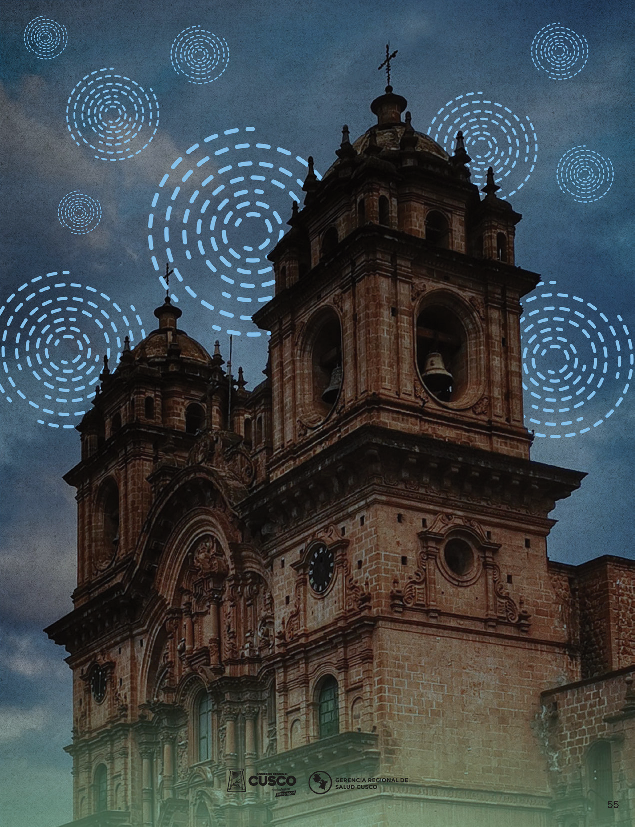
\includepdf[pages={1}]{../editorial/pagina_final.pdf}
	\clearpage
	
\end{document}